\chapter{3D-Stereokalibrierung und Szenenrekonstruktion mit reellen Daten und Kameras gleicher Auflösung}

	Bis jetzt haben wir eine Stereoanalyse und Szenenrekonstrukion in einem wie wir es nennen Minimalbeispiel durchgeführt. Hierzu wurde zum Beispiel ein Quaderobjekt definiert und dessen Eckpunkte mit Hilfe von zwei selbst definierten Kameramatrizen verrechnet so, dass ein Stereobildpaar dieses Quaders entstand. Vorteil war, dass man die korrespondierenden Punkte somit bereits besaß und die Stereoanalyse und Szenenrekonstruktion ohne Fehlerquellen wie Beispielsweise Rauschen durchführen konnte. In unserem Beispiel unter Realbedinungen, müssen zunächst die korrespondierenden Punkte des Stereobildpaares ausgemacht werden, was bis jetzt, nicht besonders präzise, von Hand funktioniert. Zu dieser Ungenauigkeit kommen dann auch noch Fehler wie Rauschen hinzu. Wie hiermit bis jetzt verfahren wird, wird folgend beschrieben.  


\section{Vorgehen}
	
Es wurde ein Stereosetup (Abbildungen 2 - 6) aufgebaut und die beiden Kameras Canon 6D und Canon 60D wurden so im Raum platziert, dass sie leicht zueinander hin gedreht waren. Die 6D wird als Ausgangskamera oder auch primär Kamera angesehen, die Position und Orientierung der 60D wird dann dementsprechend ausgehend von der 6D gemessen. Dem Voran gilt es unter anderem ein Koordinatensystem für die Canon 6D zu definieren. Danach werden die Abstände der 6D zur 60D entlang der Koordinatenachsen gemessen. Hier kann es zu deutlichen Abweichungen kommen, da von Hand mit einem Metermaß die Maße genommen wurde. Nachdem die Translation der 60D ausgehend von der 6D gemessen wurde, muss nun noch die Rotation der 60D gegenüber der 6D ermittelt werden.	

\begin{wrapfigure}{R}{0.25\textwidth}
	\centering
	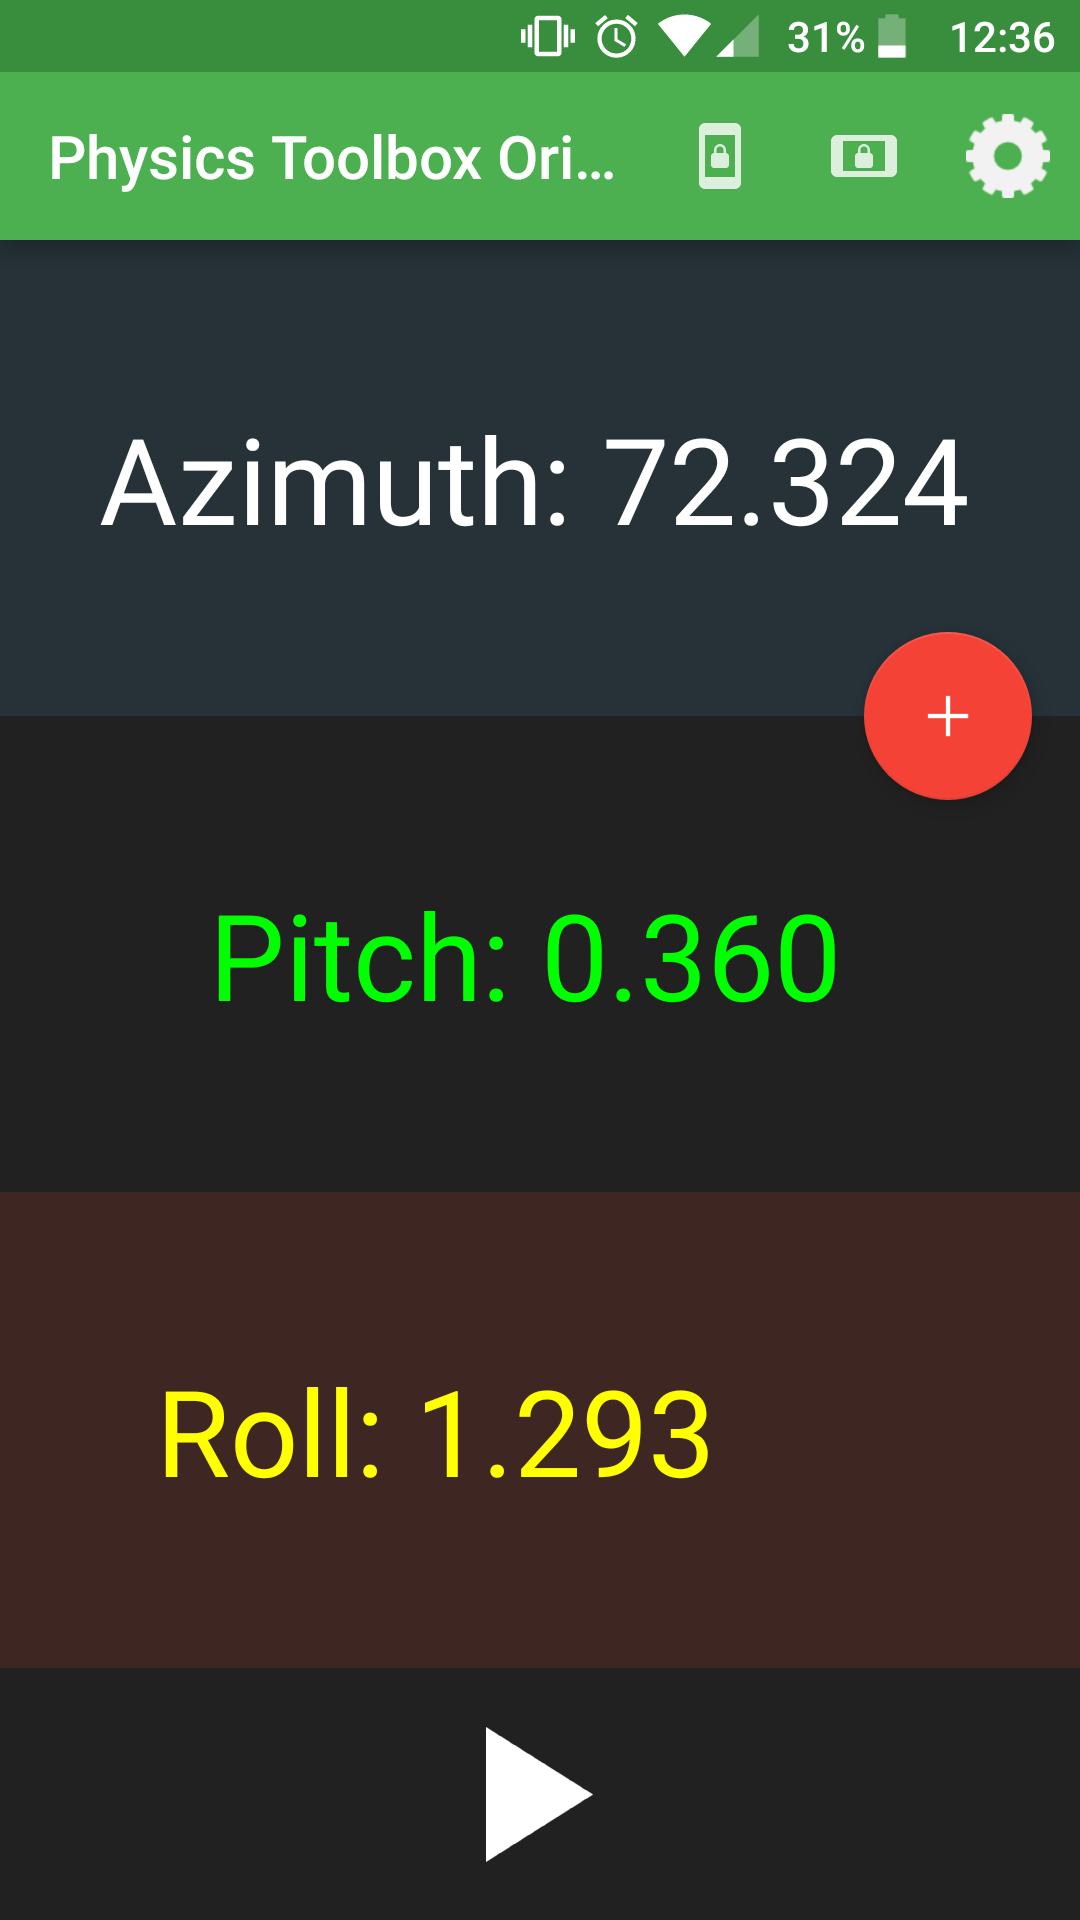
\includegraphics[width=0.25\textwidth]{Images/1_6D_Orientation_PT.png}
\end{wrapfigure}	
Da kein Gimbel zur Verfügung stand, wurde mit Hilfe einer App namens \textit{Physics Toolbox Orientation} zunächst die Orientierung der 6D ungefähr abgemessen und danach die Orientierung der 60D und die Differenz der beiden Gierwinkel der Kameras zueinander genommen um abzuschätzen wie weit die 60D zur 6D eingedreht ist. In der Toolbox gibt es den sogenannten \textit{Azimuth}-Winkel mit dessen Hilfe der Gierwinkel der beiden Kameras zueinander abgeschätzt wurde. Zur Überprüfung und weiteren Orientierung wurden zwei Metermaße auf den Boden gelegt und zwar so, dass sie quasi die Richtung der Kameramitte durch die Objektivmitte bilden. Der Schnittpunkt dieser beiden Metermaße sollte dann dazu dienen den Winkel abzumessen. Da die Metermaße nicht ganz gereicht haben, wurde ein Bild der beiden Enden so parallel wie Möglich zum Boden aufgenommen und in Geogebra die Linien der Metermaße vervollständigt, so dass der Winkel zwischen dem Schnittpunkt ausgegeben werden konnte (vgl Abbildung 1). Wie man im Protokoll sehen kann stimmen die gemessenen Winkel größtenteils überein. Rotationen um Roll- und Nickwinkel konnten leider nicht genau gemessen werden, weshalb diese auf Null gesetzt wurden. Die Daten wurden in das folgende Protokoll eingetragen.	

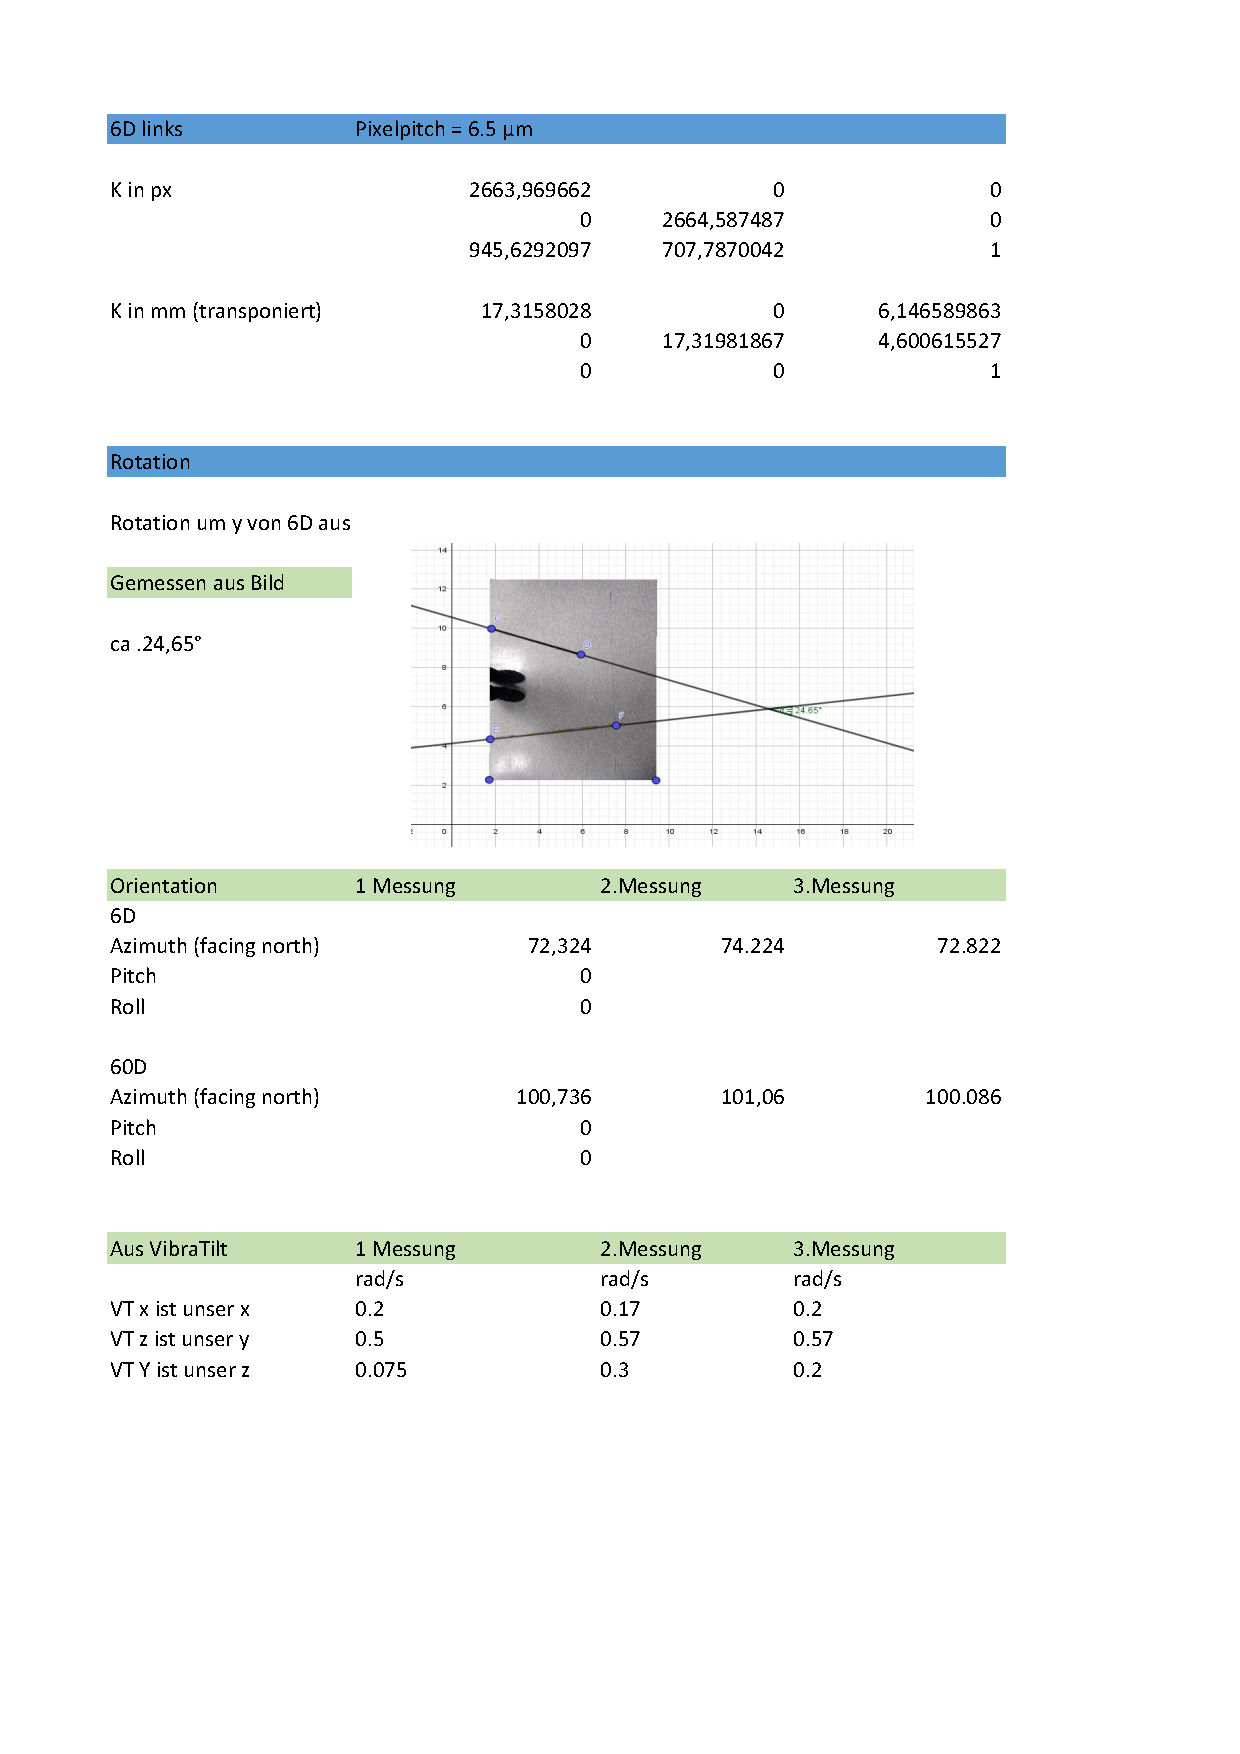
\includepdf[pages={1-},scale=1]{Images/protokoll.pdf}

\begin{minipage}{\linewidth}
	\centering
	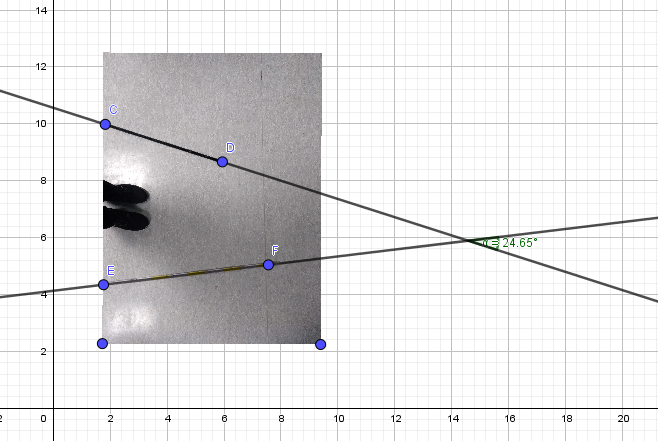
\includegraphics[width=1.\linewidth]{images/WinkelAbschaetzung.png}
	\captionof{figure}{Rekonstruktion des Gier-Winkels der Kameras zueinander}
\end{minipage}\\\\	

Mit Hilfe von Matlab wurden dann für beide Kameras Kamerakalibrierungen durchgeführt um die intrinsischen Kameramatrizen beider Kameras zu bekommen. Diese benötigen wir für die spätere Ermittlung der Essentiellen Matrix und können die Kalibrierung bis dato noch nicht selbst durchführen. Jedoch besteht hier auch die dringende Überlegung die Ermittlung der kompletten Kameramatrix allein mit der Fundamentalmatrix durchzuführen, um eine mögliche Fehlerquelle auszuschließen, weiteres zu dieser Überlegung im Unterkapitel \hyperref[sec:problem]{Probleme und mögliche Ansätze für Lösungen}  Mit den beiden Kameras wurde jeweils zeitgleich Bilder einer Szene aufgenommen (Abbildungen 5 und 6). Aus diesem Stereobildpaar wurden dann von Hand mögliche Korrespondierende Punkte rausgesucht und in Mathematica als zwei separate Punktelisten gespeichert. Nachdem alle Daten gesammelt wurden, wurde der bereits bestehende Algorithmus zur Stereokalibrierung und Szenenrekonstruktion unseres Minimalbeispiels auf die Bildpunkte angewandt. Daraufhin mussten auf Grund von fehlerhaften Resultaten bestimmte Modifizierungen vorgenommen werden, welche im Kapitel\hyperref[sec:alg]{Algorithmus} genauer beschrieben werden.
\section{Aufbau der Set-Ups}

	\begin{minipage}{\linewidth}
	\centering
	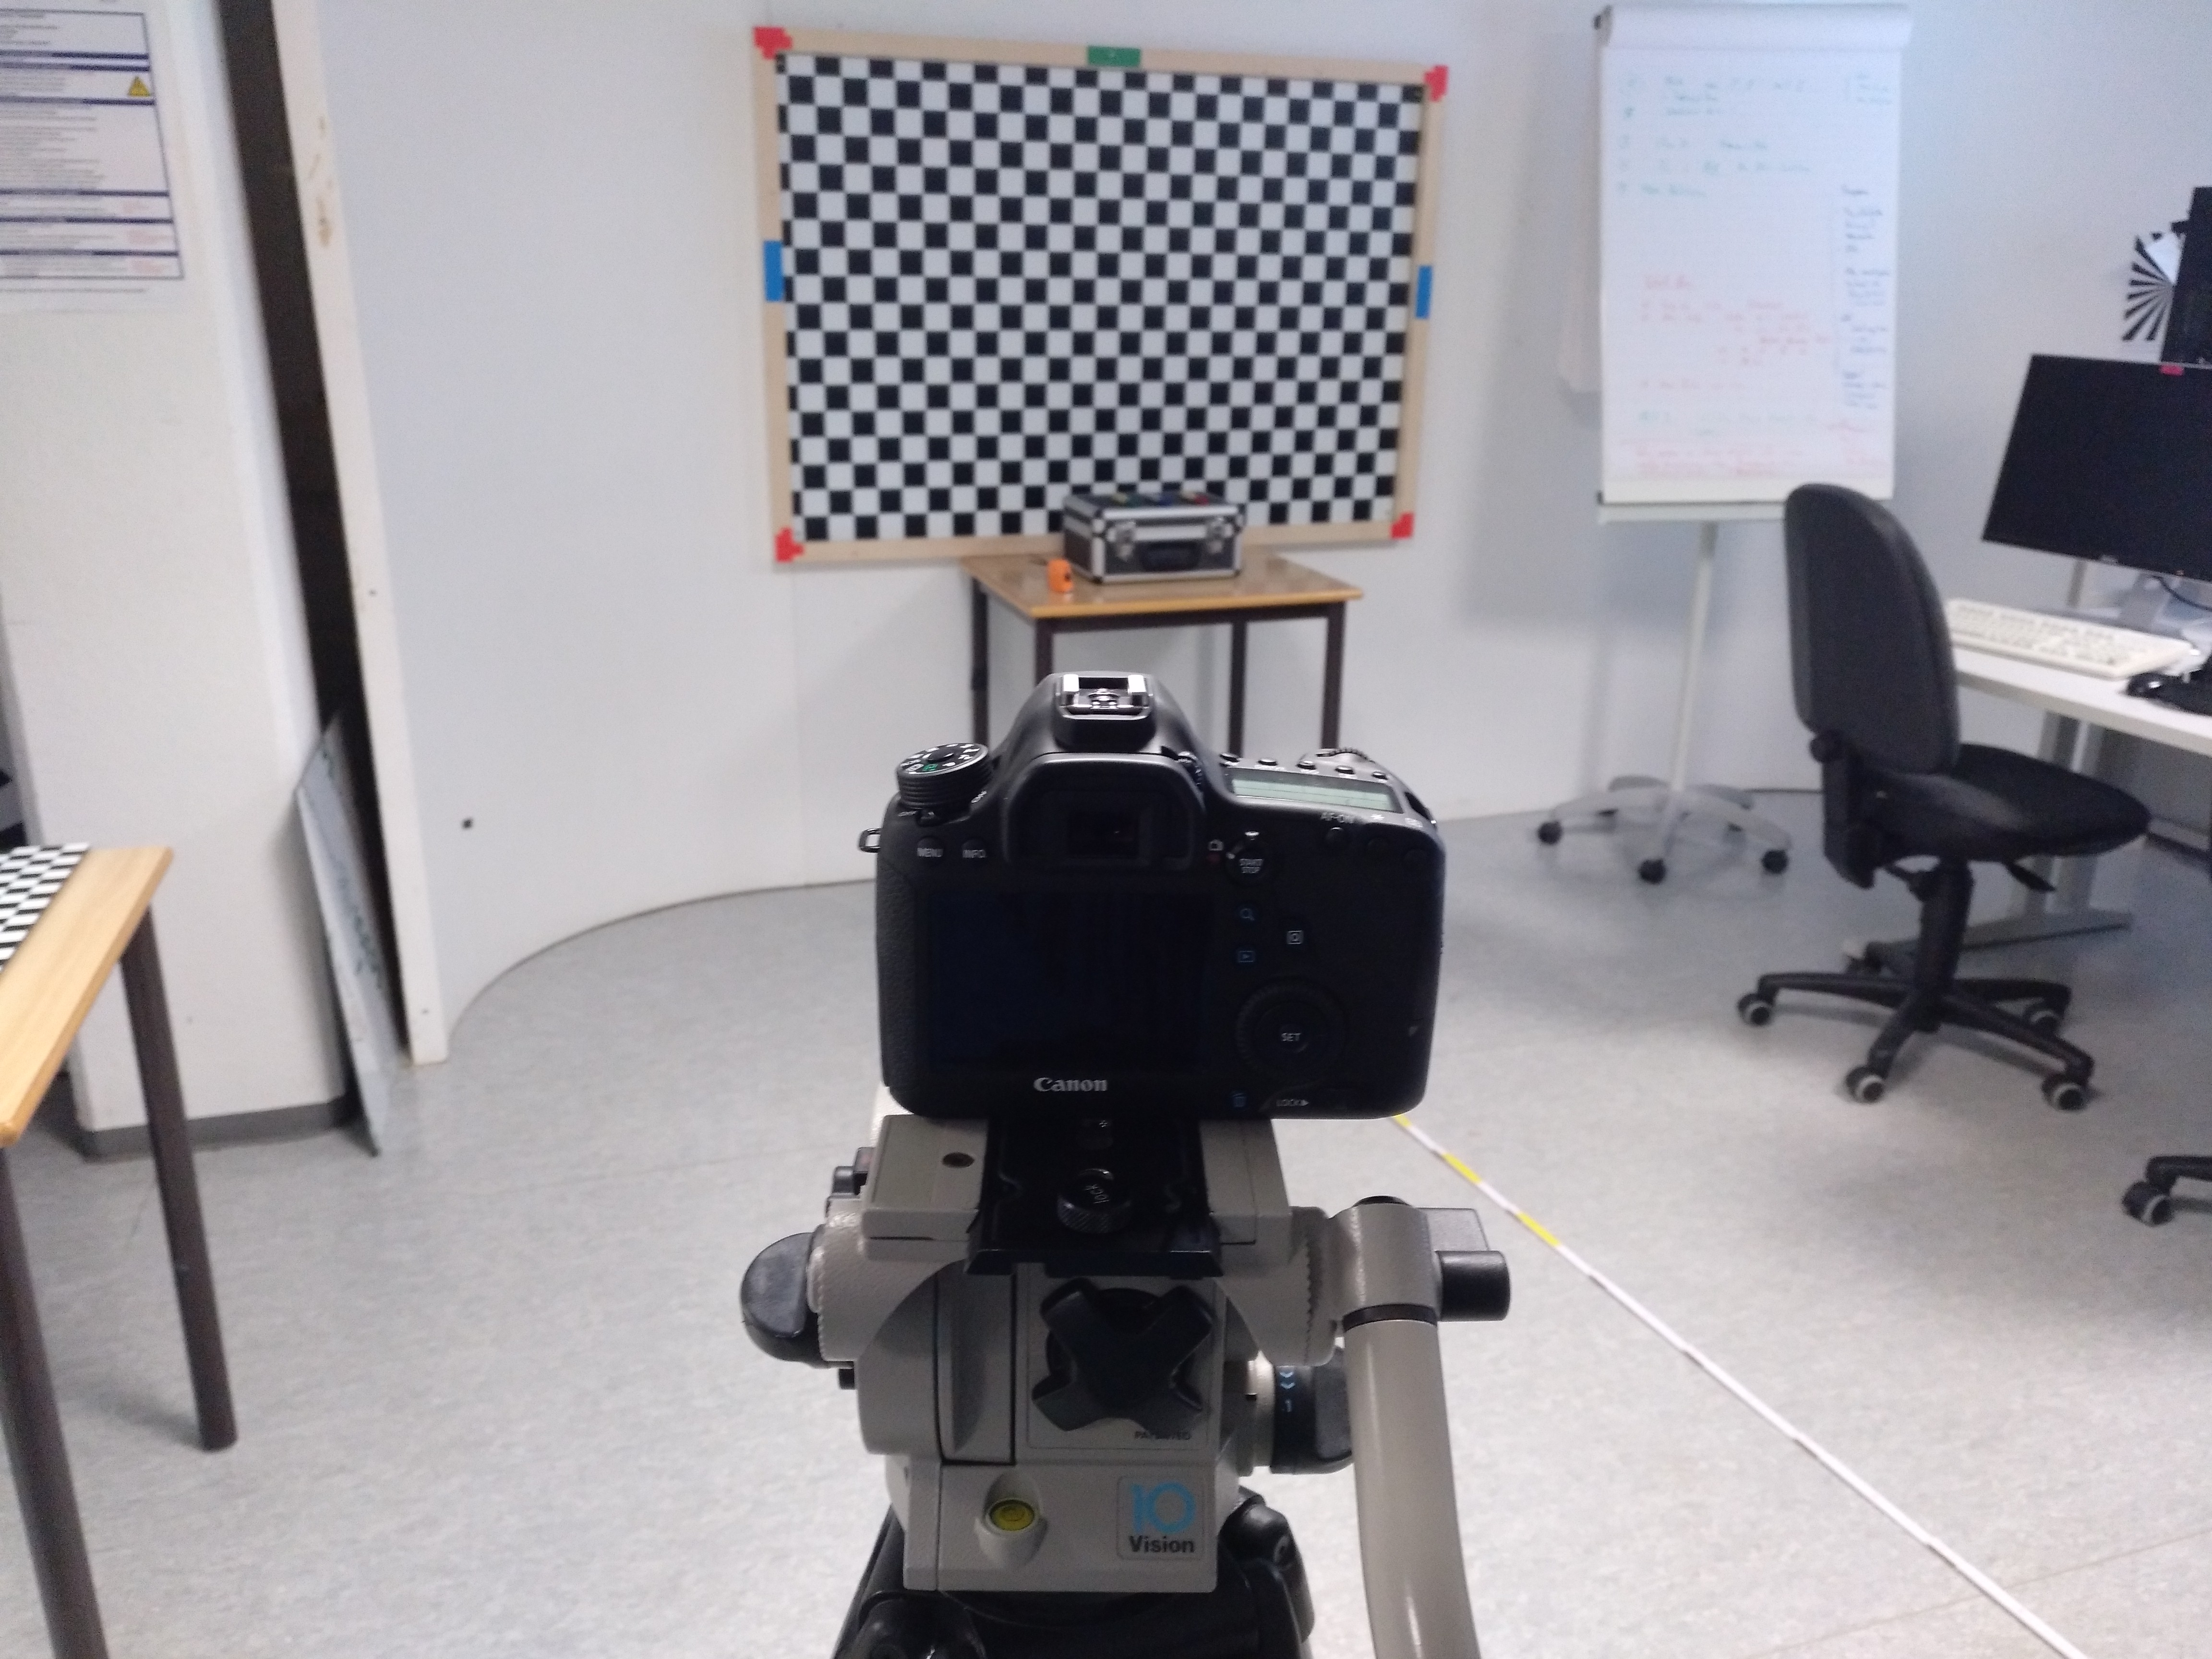
\includegraphics[width=.7\linewidth]{images/IMG_20180124_120523_760.jpg}
	\captionof{figure}{Kamera 6D}
\end{minipage}\\

\begin{minipage}{\linewidth}
	\centering
	\includegraphics[width=.7\linewidth]{images/IMG_20180124_120536_023.jpg}
	\captionof{figure}{Kamera 60D}
\end{minipage}\\

\begin{minipage}{\linewidth}
	\centering
	\includegraphics[width=.7\linewidth]{images/IMG_20180124_120502_749.jpg}
	\captionof{figure}{Stereosetup}
\end{minipage}\\

\begin{minipage}{\linewidth}
	\centering
	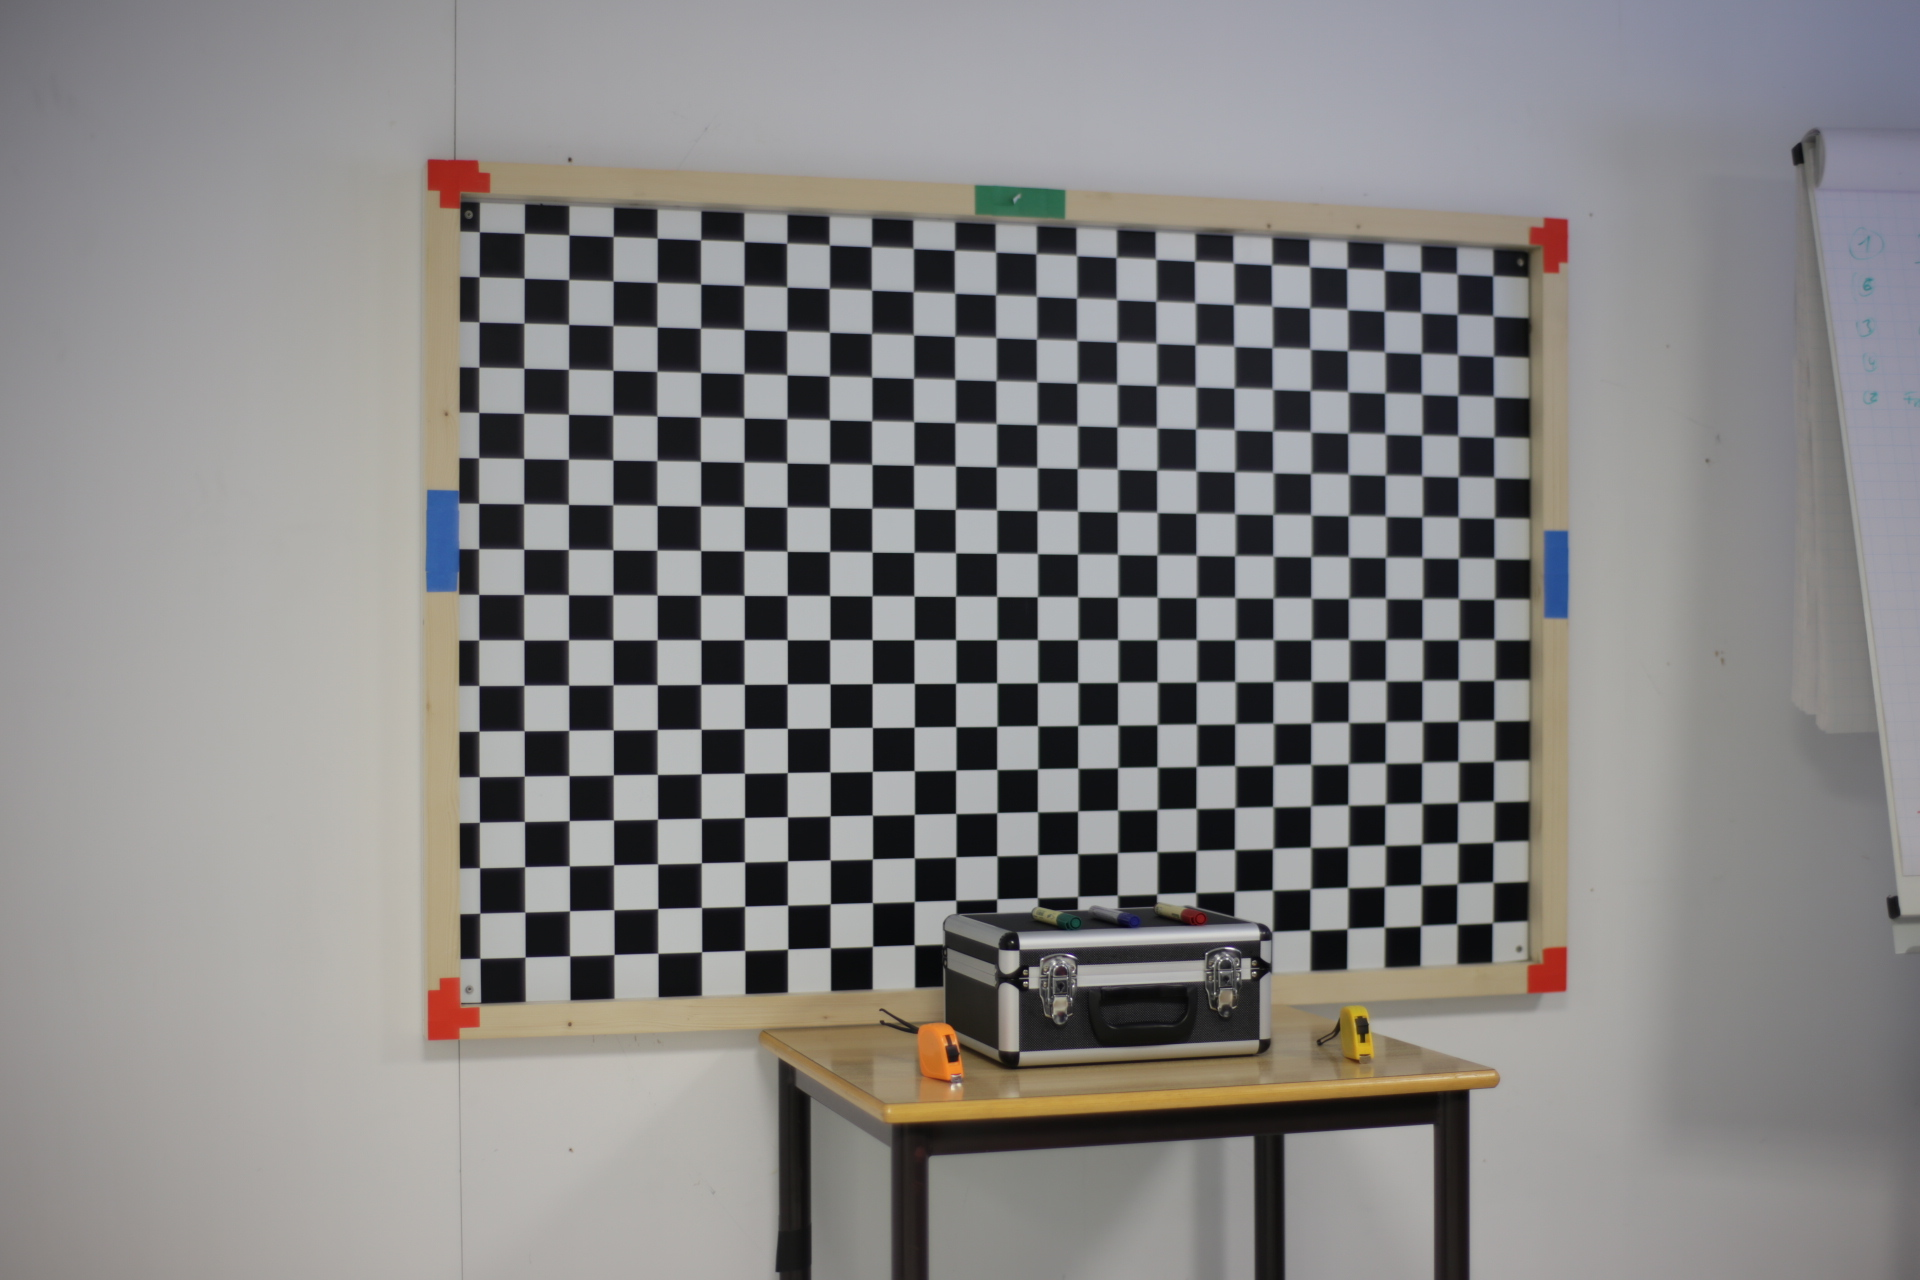
\includegraphics[width=.7\linewidth]{images/IMG_0874.jpg}
	\captionof{figure}{Szenenbild der primären Kamera 6D}
\end{minipage}\\

\begin{minipage}{\linewidth}
	\centering
	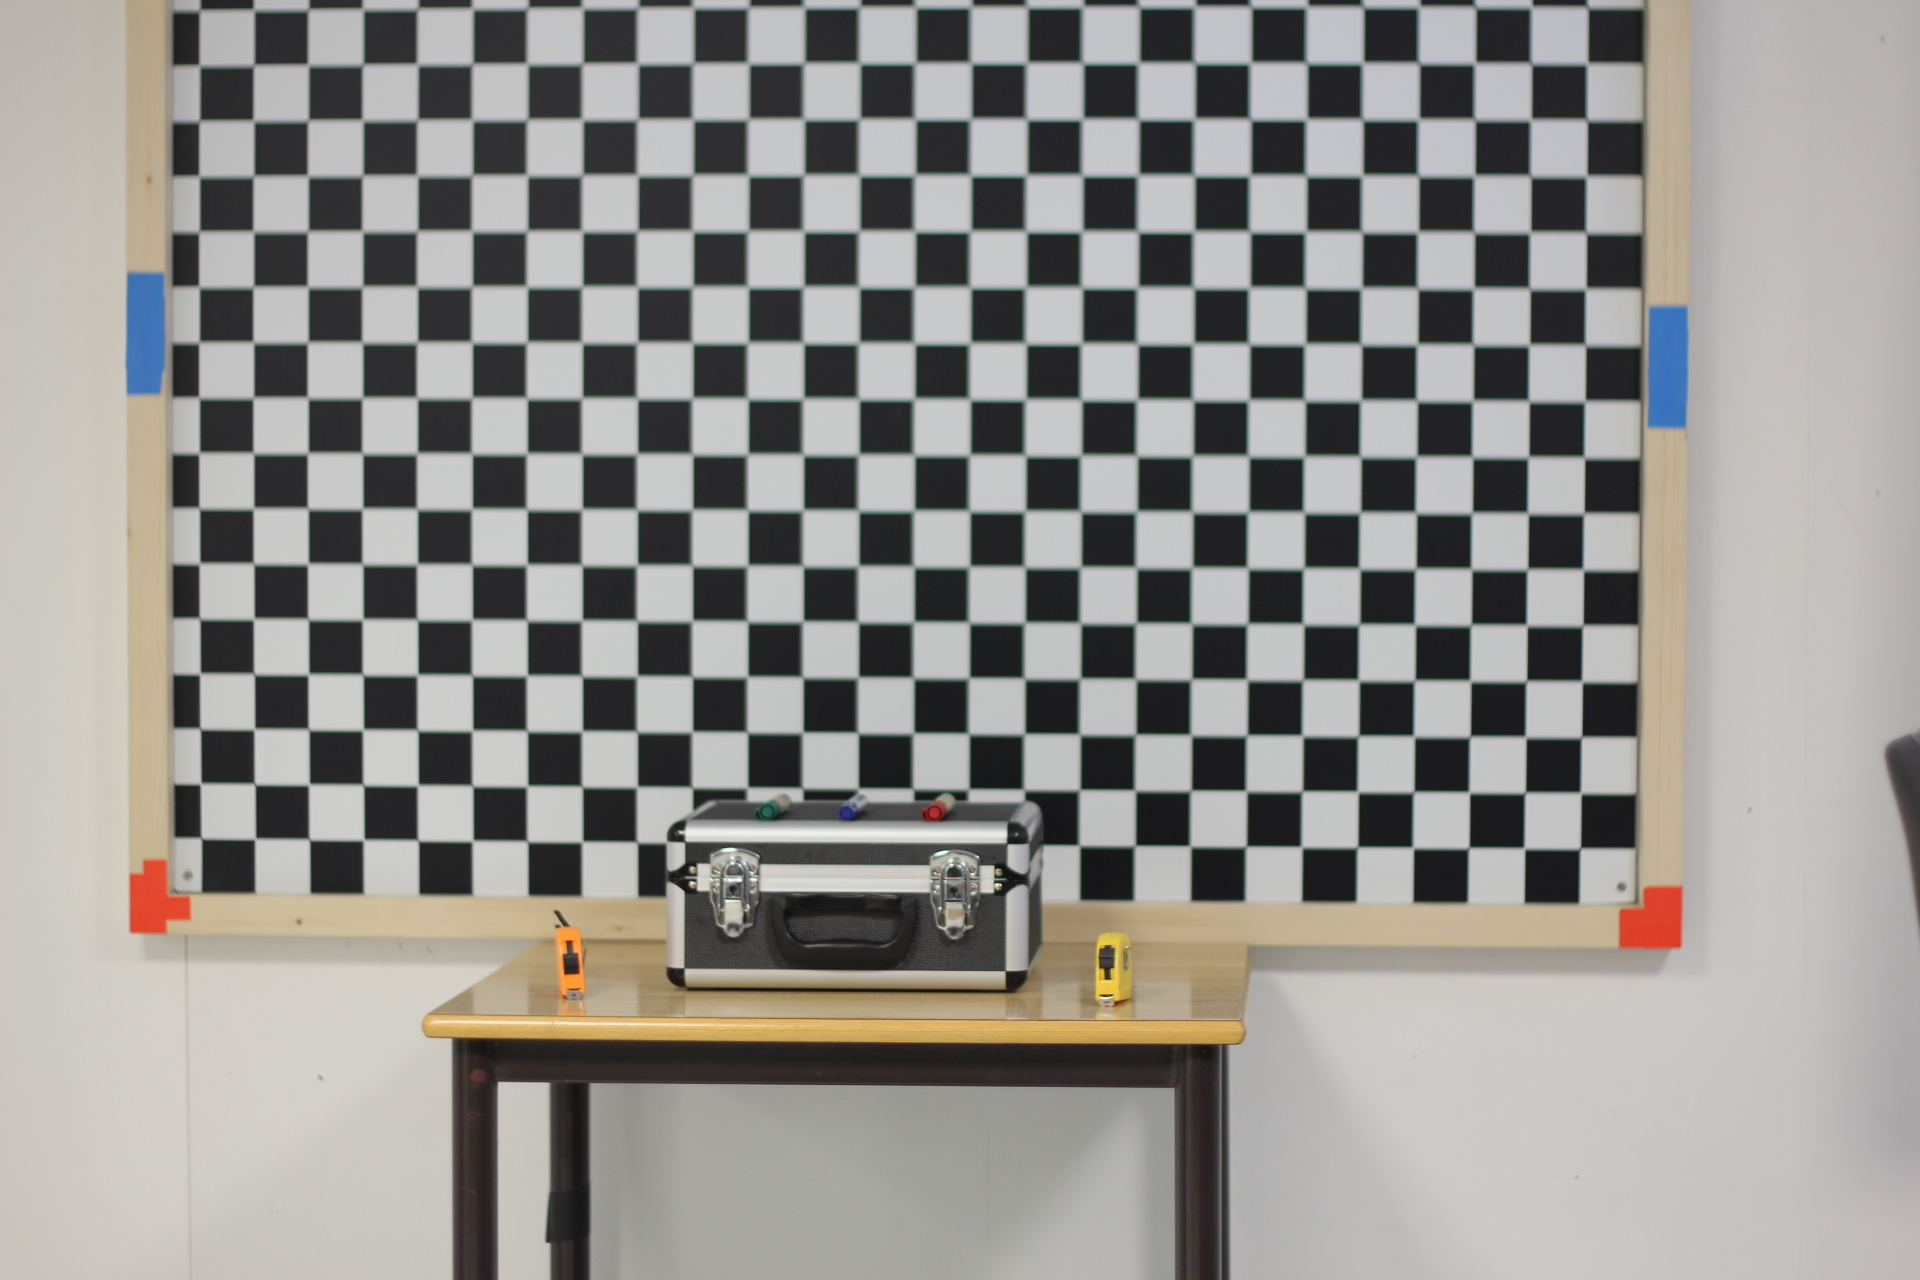
\includegraphics[width=.7\linewidth]{images/IMG_5434.jpg}
	\captionof{figure}{Szenenbild der sekundären 60D}
\end{minipage}\\

\section{Unterschiede im Algorithmus im Verlgleich zum Minimalbeispiel}

\textit{StereoAnalyse.nb} beinhaltet den kompletten Code von der Ermittlung der Fundamentalmatrix über die Umrechnung in die essentiellen Matrix und letztendlich die Rekonstruktion der externen Kameraparameter. Die Datei \textit{Points\_SetUp.nb} beinhaltet die ausgelesenen korrespondierenden Punkte und die Ergebnisse der Berechnungen werden in der Datei \textit{results.nb} angezeigt. \\

Der erste Schritt des Algorithmus beinhaltet die Ermittlung der Fundamentalmatrix mit dem normalized-8-Point-Algorithm. Die Entscheidung den normalized-8-Point-Algorithm  zu benutzen fiel als festgestellt wurde, dass ohne vorherige Normalisierung der ausgelesenen Punkte es zu größeren Fehlern in den weiteren Berechnungen kam. Zur Erklärung dieser Fehler kann zum einen die \textit{Condition Number} betrachten \cite{HZ8}, welche in der \textit{SVD} der entstehenden Matrix aus der Koeffizientenmatrix mit ihrer transponierten ausgelesen werden kann. Diese sollte möglichst klein sein, jedoch ist sie bei nicht normalisierten Koordinaten relativ hoch. Der Grund für den nicht optimalen Wert der \textit{Condition Number} ist das Fehlen der Homogenität in den Bildkoordinaten.\cite{HZ8}. Die weitere Erklärung findet sich im Paper von Richard I. Hartely unter Kapitel 4. Hinzuzufügen ist noch, dass je größer die \textit{Condition Number} ausfällt, desto größer wirken sich kleinste Abweichungen der Daten wie beispielsweise Rauschen in den Bildern auf die Resultate aus. \\







\subsection{normalisierung der eingehenden Daten und Berechnung der Fundamentalmatrix über den normalized 8-Point-Algorithm}


Nach diesem Exkurs zurück zum Algorithmus. Die Bildpunkte werden also zu aller erst Normalisiert. Hierzu wurde ein Modul geschrieben, welches für die Bildpunktpaare beider Bilder zwei Matrizen aufstellt, die eine Skalierung und Translation der Punkte des jeweiligen Bildes bewirkt. Normalisieren bedeutet in diesem Falle, dass die Schwerpunkt der Punktewolken pro Bild ermittelt wurden und diese dann in den Ursprung des jeweiligen Bildes verschoben wurden, danach wurden die Punkte ebenfalls mit Beibehaltung ihres Abstandsverhältnisses zum Schwerpunkt mit verschoben. Als nächstes wurde der Durchschnittsabstand der Punkte zum neu gelegenen Schwerpunkt auf \ensuremath{\sqrt{2}} gebracht. Die entstandenen Punkte befinden sich nun in einem deutlich kleineren Zahlenbereich als zuvor meist zwischen ca -1 und 1. danach werden diese normierten Punkte an ein Modul namens \textit{FundamentalMtxBestimmung} übergeben zusammen mit den beiden Normalisierungsmatritzen \textit{T} und \textit{T'}, welche später für die Denormalisierung der Fundamentalmatrix erneut benötigt werden.\\

Im Modul \textit{FundamentalMtxBestimmung} wird eine Koeffizientenmatirx nach den Vorgaben aus \textit{Hartley and Zisserman} erstellt\cite{HZ}. 

\begin{gather}
x'^T F x =0\\
F=\begin{bmatrix}
f_{11}&f_{122}&f_{13}\\
f_{21}&f_{22}&f_{23}\\
f_{31}&f_{32}&f_{33}
\end{bmatrix}\\
\begin{pmatrix}
x'_n&y'_n&1
\end{pmatrix} 
\cdot
\begin{bmatrix}
f_{11}&f_{122}&f_{13}\\
f_{21}&f_{22}&f_{23}\\
f_{31}&f_{32}&f_{33}
\end{bmatrix}
\cdot
\begin{pmatrix}
x_n\\y_n\\1
\end{pmatrix} =0\\
f_{11}x_nx'_n+f_{12}y_nx'_n+f_{13}x'_n+f_{21}x_ny'_n+f_{22}y_ny'_n+f{23}y'_n+f_{31}x_n+f_{32}y_n+f_{33} =0\\
(x_nx'_n,y_nx'_n,x'_n,x_ny'_n,y_ny'_n,y'_n,x_n,y_n,1)\cdot f =0\\
\begin{bmatrix}
x_1x'_1&y_1x'_1&x'_1&x_1y'_1&y_1y'_1&y'_1&x_1&y_1&1\\
x_2x'_2&y_2x'_2&x'_2&x_2y'_2&y_2y'_2&y'_2&x_2&y_2&1\\
.&.&.&.&.&.&.&.&.\\
.&.&.&.&.&.&.&.&.\\
.&.&.&.&.&.&.&.&.\\
x_nx'_n&y_nx'_n&x'_n&x_ny'_n&y_ny'_n&y'_n&x_n&y_n&1
\end{bmatrix}
\cdot 
\begin{pmatrix}
f_{11}\\f_{12}\\f_{13}\\f_{21}\\f_{22}\\f_{23}\\f_{31}\\f_{32}\\f_{33}
\end{pmatrix}
= 0
\end{gather}\\

Im Idealfall und auch in unserem Fallbeispiel ist der Rang dieser Koeffizientenmatrix bei 8, jedoch durch Ungenauigkeiten der Bildpunkte durch Rauschen und da es sich um einen überbestimmten Fall mit mehr also nur acht korrespondierenden Punkten handelt ist der Rang bei 9, weshalb wenn man sich den Kern dieser Matrix ausgeben lässt, man für \textit{F} keine Eindeutige Lösungen bekommt. 

\begin{minipage}{\linewidth}
	\centering
	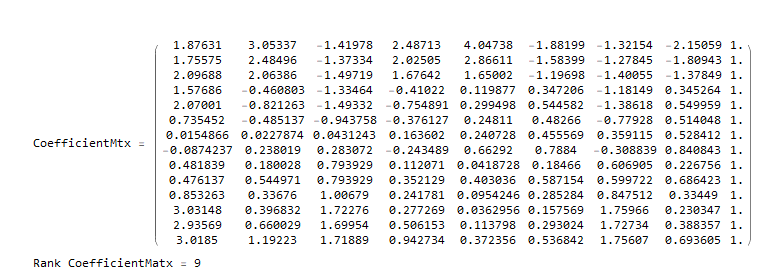
\includegraphics[width=1\linewidth]{images/KoefficientMtx.png}
	\captionof{figure}{Beispiel einer resultierenden Koeffizientenmatrix}
\end{minipage}\\

Aus diesem Grund beschaffen wir uns die Fundamentalmatrix etwas anders. Es wird eine \textit{SVD} der Koeffizientematrix durchgeführt, um eine \textit{least-square-solution} zu finden. Die \textit{least-square-solution} für \textit{f} ist der Singulärvektor entsprechend dem kleinsten Singulärwert der Koeffizientenmatrix, welcher der letzten Spalte von \textit{V} entspricht. Die Fundamentalmatrix ist hiermit aber noch nicht vollständig bestimmt. Das Resultierende \textit{F} hat nämlich den Rang 3 und ist somit keine gültige Fundamentalmatrix. Diese muss singulär sein und den Rang 2 besitzen. Es muss also ein \textit{singularity-constraint} erzwungen werden, welcher uns eine Fundamentalmatrix \textit{\^F} mit Rang 2 aus \textit{F} ermittelt. Das Problem ist nämlich, dass wenn wir mit \textit{F} uns Beispielsweise die Epipolarlinien ausrechnen wir folgende Plots der beiden Bilder erhalten.\\


\begin{minipage}{\linewidth}
	\centering
	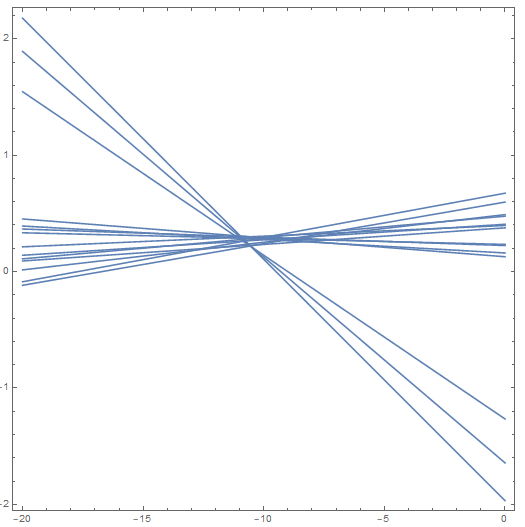
\includegraphics[width=.8\linewidth]{images/LinesF6D.png}
	\captionof{figure}{Resultierende Epipolarlinien des Bildes der Canon 6D}
\end{minipage}
\begin{minipage}{\linewidth}
	\centering
	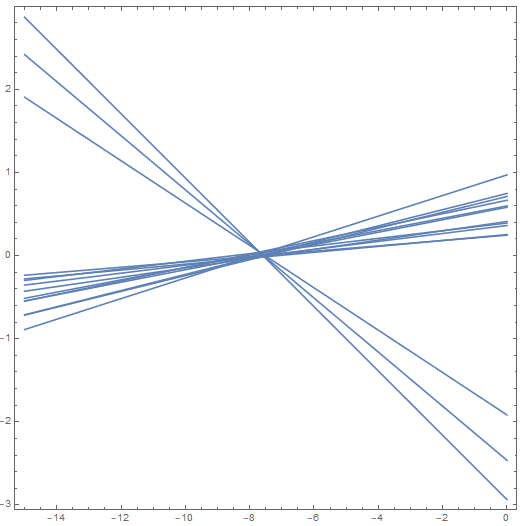
\includegraphics[width=.8\linewidth]{images/LinesF60D.png}
	\captionof{figure}{Resultierende Epipolarlinien des Bildes der Canon 60D}
\end{minipage}\\

Wie man auf den Bildern erkennen kann, treffen sich die Epipolarlinien nicht in einem Epipol. Die Erzwingung einer Singularität von \textit{F} soll dieses Problem beheben. Auch hier halten wir uns an das Verfahren welches im \textit{Hartley und Zisserman} \cite{HZ} beschrieben wird. Wir führen an \textit{F} eine \textit{SVD} durch und bekommen \textit{F} in \textit{\ensuremath{UDV^T}} zerlegt. \ensuremath{D} beinhaltet in einer diagonalen Matrix die Singulärwerte \ensuremath{D = \text{diag}(r,s,t)}, welche die Bedingung \ensuremath{r \leq s \leq t } erfüllen. Um den \textit{singularity-constraint} zu erzwingen, setzen wir den letzten Singulärwert \ensuremath{t = 0} und erhalten somit \ensuremath{D = \text{diag}(r,s,0)}. Danach wird \textit{\^F} wieder zusammmengesetzt mit dem modifizierten \ensuremath{D} und bekommen \ensuremath{\textit{\^F} = UDV^T} welches die Frobenius-Norm von \ensuremath{F-\textit{\^F}} minimiert \cite{HZ}. Das neue \textit{\^F} führt, wenn wir uns wieder die Epipolarlinien ausgeben lassen zu folgendem Ergebnis.


\begin{minipage}{\linewidth}
	\centering
	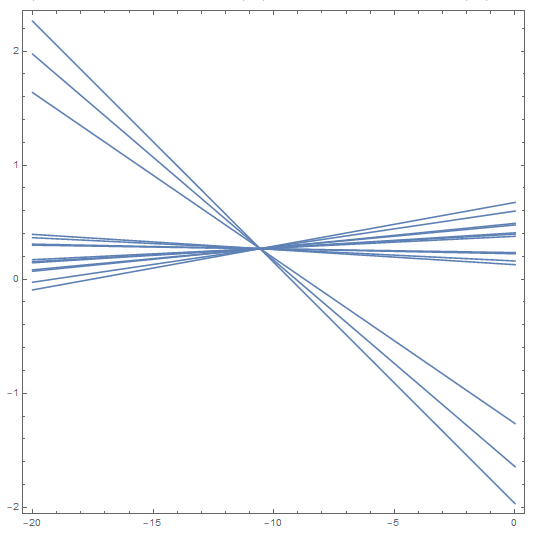
\includegraphics[width=.8\linewidth]{images/LinesFPrime6D.png}
	\captionof{figure}{Resultierende Epipolarlinien des Bildes der Canon 6D nach singularity-constraint}
\end{minipage}
\begin{minipage}{\linewidth}
	\centering
	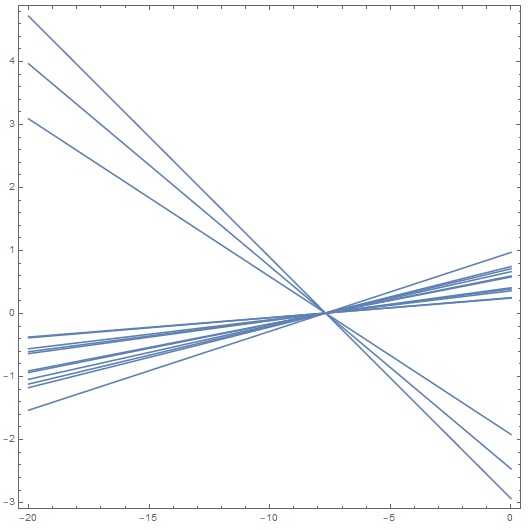
\includegraphics[width=.8\linewidth]{images/LinesFPrime60D.png}
	\captionof{figure}{Resultierende Epipolarlinien des Bildes der Canon 60D nach singularity-constraint}
\end{minipage}\\

Letztendlich wird dann \textit{\^F} noch mit Hilfe der beiden Matrizen \textit{T} und \textit{T'} denormalisiert 

\begin{gather}
F = T'\,^T\textit{\^F}T
\end{gather}
\subsection{Ermitteln der Essentiellen Matrix und Einführung des singularity-constraints}

Mit dieser Fundamentalmatrix und den aus Matlab erlangten internen Kamerparametern \ensuremath{K_1} der Canon 6D und \ensuremath{K_2} der Canon 60D kann nun auf zwei Verschiedene Weisen die essentielle Matrix berechnet werden. Hier werden beide Vorgänge kurz erläutert aber mit dem Vorbehalt, dass die essentielle Matrix in unserem Realbeispiel wohl nicht gänzlich korrekt ist, da diese uns nicht die gewünschten Resultate liefert. Mehr dazu später.\\

In der Theorie kann die Essentielle Matrix durch Verrechnung der beiden Kameramatrizen \ensuremath{K_1} und \ensuremath{K_2} mit der denormalisierten Fundamentalmatrix \textit{F} erschlossen werden.

\begin{gather}
E = K_2^TFK_1
\end{gather} 

Zum anderen kann man aber auch so vorgehen wie bei der Berechnung der Fundamentalmatrix nur müssen hierzu die Koordinaten zunächst von Pixel in Millimeter umgerechnet werden und danach noch mit den Kameramatrizen normalisiert werden. Ist dies erfolgt kann das selbe Verfahren wie bei der Fundamentalmatrix mit dem \textit{8-Point-Algorithm} angewandt werden.\\

Schon nach Berechnung der essentiellen Matrix zeigt sich in unserem Beispiel eine Ungenauigkeit. Denn bei der Überprüfung ob gilt dass:

\begin{gather}
\text{\^x'}E\text{\^x} = 0
\end{gather}\\

Kommt es doch zu einer nicht ignorierbaren Ungenauigkeit. Die Werte befinden sich in einem Bereich zwischen -0.3 und -0.7. Betrachtet man von \ensuremath{E} die \textit{SVD}, so wird ersichtlich, dass sie ersten beiden Singulärwerte nicht identisch sind, was aber bei einer gültigen Essentiellen Matrix der Fall sein muss \cite{HZ}. Auch hier wird einem nahegelegt diesen \textit{constraint} zu erzwingen. \textit{E} wird durch die \textit{SVD} in \ensuremath{E = UDV^T} zerlegt. Auch hier sind die Singulärwerte in der Diagonalmatrix \ensuremath{D = \text{diag}(a,b,c)} mit \ensuremath{a\leq b \leq c} gegeben. Um nun den gewünschten \textit{singularity-constraint} zu erwirken wird \ensuremath{D} folgendermaßen modifiziert. \textit{\^D} = diag \ensuremath{\frac{a+b}{2}},\ensuremath{\frac{a+b}{2}},0. Danach wird \textit{\^E} wieder zusammengesetzt mit \ensuremath{\textit{\^E}= UDV^T}. Doch trotzdem haben sich die Resultate kaum gebessert wie man in  Abblidung 12 sehen kann.\\

\begin{minipage}{\linewidth}
	\centering
	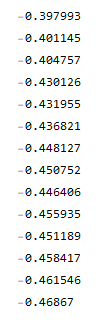
\includegraphics[width=.15\linewidth]{images/resultE.png}
	\captionof{figure}{Ergebnis der Prüfung der Punktekorrespondenzen mit der essentiellen Matrix}
\end{minipage}\\\\

Auch den Versuch das Verfahren mit den bereits normalisierten Koordinaten für die Berechnung der Fundamentalmatrix zu verwenden oder die essentielle Matrix aus der nicht denormalisierten Fundamentalmatrix zu berechnen, hat leider keine Besserung des Ergebnisses erzielt. Vermutet werden kann, dass die ausgelesenen korrespondierenden Punkte vielleicht doch viel zu ungenau sind oder die Bilder gar leicht Verzeichnet sind, was zu einer Anhäufung der Fehler führen könnte. Nichtsdestotrotz wurde der Algorithmus weitergeführt und versucht die Rotation und Translation der Canon 60D zur 6D zu ermitteln. Hierzu wurde sich ebenfalls an dem Verfahren aus dem Buch von \textit{Hartley and Zisserman} orientiert.\\

\section{Rekonstruktion der exterenen Kameraparameter}
Dem Modul \textit{ExtractRotationAndTranslation} wird die Essentielle Matrix übergeben. Um nun die äußeren Kameraparameter zu bestimmen, muss zunächst die essentielle Matirx \ensuremath{E} mit Hilfe der \textit{SVD} zerlegt werden. Das Ergebnis sind drei Matrizen der Form 

\begin{gather}
E = U\Sigma V^T
\end{gather}

Zu Beachten ist dass die Essentielle Matrix so angepasst werden muss dass am besten für \ensuremath{\Sigma} gilt:

\begin{gather}
\Sigma = diag(1,1,0)
\end{gather}

Was zuvor durch den \textit{constraint} erwirkt wurde.Wir wissen dass:

\begin{gather}
E=[t]_xR\\
S =[t]_x\\
E=SR
\end{gather}

Zur Unterstüzung der Berechnung der externen Kameraparameter nehmen wir die Matrizen \ensuremath{W} und \ensuremath{Z} zu Hilfe. In Hartley and Zisserman, kann man im Appendix auf Seite 541 den genaueren Ursprung dieser beiden Hilfsmatrizen erfahren\cite{HZ}.

\begin{gather}
W = \begin{pmatrix}
0&-1&0\\
1&0&0\\
0&0&1
\end{pmatrix} \;\;\;
Z=
\begin{pmatrix}
0&1&0\\
-1&0&0\\
0&0&0
\end{pmatrix}
\end{gather}

Mit dem Ergebnis der \textit{SVD} von \ensuremath{E} lassen sich nun jeweils zwei Ergebnisse für S und R finden:	

\begin{gather}
S_1 = -UZU^T \;\;\;\; R_1 = UW^TV^T\\
S_2 = UZU^T \;\;\;\; R_2 = UWV^T
\end{gather}\\

Um sicher zu gehen, dass es sich bei \ensuremath{R_1} und \ensuremath{R_2} auch um Rotationen handelt, kann man folgende Proben durchführen. Zum einen muss \ensuremath{R\cdot R^T=I_{3x3}} sein. \ensuremath{I_{3x3}} bezeichnet in diesem Fall eine 3x3-Einheitsmatrix. Des Weiteren kann man überprüfen, ob die Determinante \ensuremath{det(R_1) = 1} ist. Nun müssen wir aus den 3x3-Matrizen \ensuremath{S_1} und \ensuremath{S_2} noch das fehlende \ensuremath{t} rausfiltern. Wir wissen:

\begin{gather}
St = [t]_x \cdot t = t \times t
\end{gather} 

Daraus kann man schließen, dass \ensuremath{t} = dem Nullspace von \ensuremath{S_1} und \ensuremath{S_2} ist. Der Nullspace beider Matrizen \ensuremath{S_1} und \ensuremath{S_2} ist der selbe. Die externen Kameraparameter lassen sich wie gesagt nur bis zu einem Skalierungsfaktor genau berechnen. Dass soll heißen, ist \ensuremath{t} der Nullspace von \ensuremath{S_1} und \ensuremath{S_2}, so ist auch das Vielfache \ensuremath{\lambda t} eine gültige Lösung für t. Letzten Endes haben wir für die externen Kameraparameter vier verschiedene Lösungen. 

\begin{gather}
PM2 = [UWV^T|+\lambda t] \;\;\; oder \;\;\;[UW^TV^T|+\lambda t]\\
or\;\;\; [UWV^T|-\lambda t] \;\;\; oder \;\;\;[UW^TV^T|-\lambda t]
\end{gather}\\

Bei den Bestimmungen der externen Kameraparameter kommt es dann zu weiteren Unstimmigkeiten. So sollte zum Beispiel der linke Nullspace von \textit{E} und \textit{S} das selbe Ergebnis aufzeigen. Jedoch unterscheiden sich beide Ergebnisse leicht voneinander \\

\begin{minipage}{\linewidth}
	\centering
	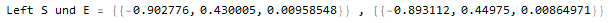
\includegraphics[width=1\linewidth]{images/LeftES.png}
	\captionof{figure}{Linker Nullspace von E und S}
\end{minipage}\\\\

Zudem sollte aus den Ergebnissen resultieren, dass \ensuremath{E = [t]_xR} ist und somit das Ergebnis mit unserem \textit{E}, welches wir dem Modul übergeben übereinstimmt. Auch hier kommt es zu Unstimmigkeiten.\\

\begin{minipage}{\linewidth}
	\centering
	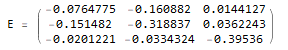
\includegraphics[width=.4\linewidth]{images/E.png}
	\captionof{figure}{Übergebene Essentielle Matrix}
\end{minipage}\\\\

\begin{minipage}{\linewidth}
	\centering
	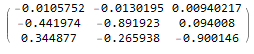
\includegraphics[width=.4\linewidth]{images/TestE.png}
	\captionof{figure}{Test \ensuremath{E = [t]_xR}}
\end{minipage}\\\\

Und letztendlich kommen für Rotation und Translation nicht die gewünschten Ergebnisse welche im Protokoll notiert waren raus. Außerdem stimmen sie nicht hundertprozentig mit der zur Probe in Matlab durchgeführten Stereokalibrierung überein.
\section{Szenenrekonstruktion mit Hilfe der Sampson-approximation}
\subsection{andere Ansätze für Triangulationsverfahren}



